%%%% Realisering af tab efter optimerng %%%%

\subsection{Tab}
Det nye tab i converteren er estimeret ved samme fremgangsmåde som i 2. iteration. Dette blev gjort ved måling af temperaturstigningen i kølepladen. Det eneste ændrede ved 3. iteration der påvirker tabet i converteren, er switch-tiden i MOSFET'en, derfor er det også det eneste måles i dette afsnit. Der vil igen regnes en endelig effektivitet i converteren, ved både lav og høj indgangsspænding. 

Temperaturen i MOSFET'en er målt på figur~\ref{fig:mosfet_tab_3}. Her er det aflæst til $46.3\degreeCelsius$. Det giver en temperaturstigning på $46.3\degreeCelsius - 25\degreeCelsius = 21.3\degreeCelsius$. Ud fra dette kan effektafsættelsen i MOSFET'en regnes.

\begin{equation}
P_{diode} = \frac{21.3\degreeCelsius}{9.5K/W} = 2.29W
\end{equation}


\begin{figure}[H]
	\center
	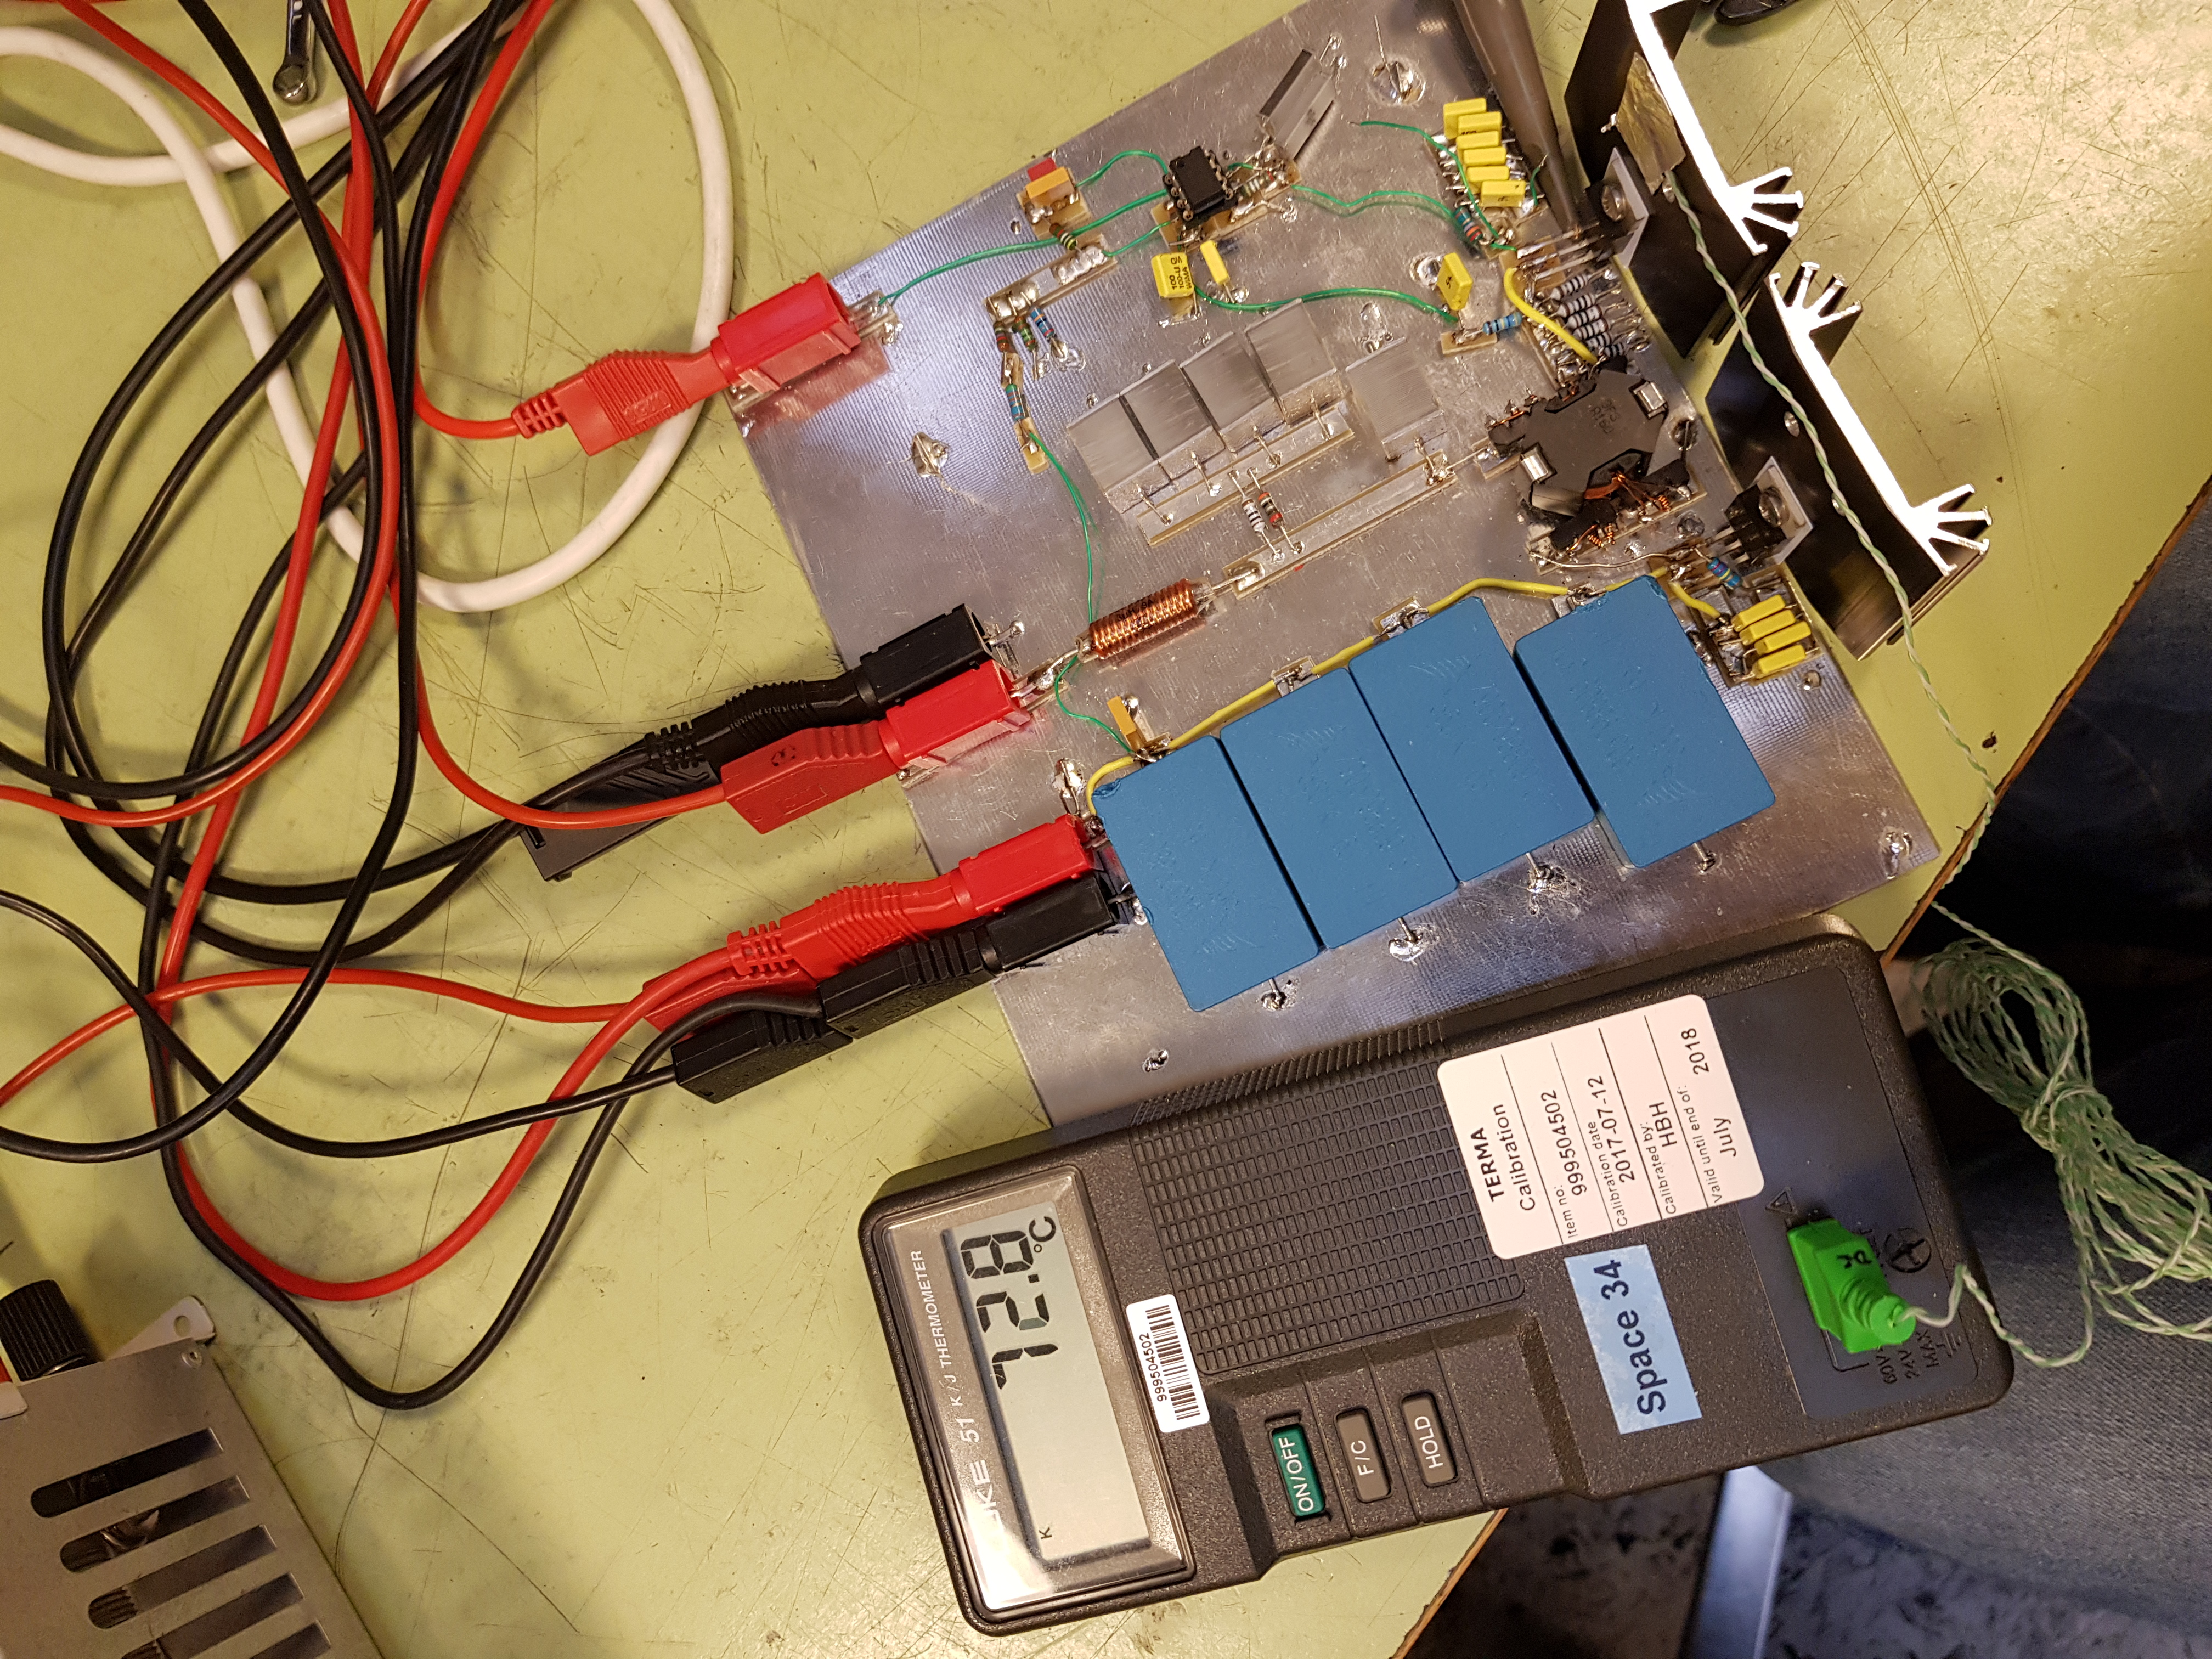
\includegraphics[max width=0.7\linewidth]{/tex/3iteration/billeder/Realisering/MOSFET.jpg}
	\caption{Temperatur i MOSFET køleplade}
	\label{fig:mosfet_tab_3}
\end{figure}

Converterens effektivitet regnes ved forholdet mellem udgangseffekten og indgangseffekten. Disse findes ved, at måle strømme og spændinger på indgang og udgang. Indgangseffekten, udgangseffekt og effekttab regnes ved følgende ligninger.

\begin{equation}
P_{in} = V_{in} \cdot I_{in} = 26V \cdot 2.3A = 59.8W
\end{equation}

\begin{equation}
P_{out} = V_{out} \cdot I_{out} = 20.99V \cdot 2.57A = 53.9W
\end{equation}

\begin{equation}
P_{loss} = P_{in} - P_{out} = 59.8W - 53.9W = 5.9W
\end{equation}

\noindent Ud fra indgangs- og udgangseffekten regnes også den endelige effektivitet i converteren. 

\begin{equation}
\eta = \frac{P_{out}}{P_{in}} \cdot 100 = \frac{53.9W}{59.8W} \cdot 100 = 90.21\percent
\end{equation}

\noindent Samme beregninger er foretaget ved en indgangsspænding på $50V$.
\begin{equation}
P_{in} = V_{in} \cdot I_{in} = 50V \cdot 1.1A = 55W
\end{equation}

\begin{equation}
P_{out} = V_{out} \cdot I_{out} = 20.99V \cdot 2.5A = 52.5W
\end{equation}

\begin{equation}
P_{loss} = P_{in} - P_{out} = 55W - 52.5W = 2.5W
\end{equation}

\begin{equation}
\eta = \frac{P_{out}}{P_{in}} \cdot 100 = \frac{52.5W}{55W} \cdot 100 = 95.4\percent
\end{equation}



Resultaterne indsættes i tabel~\ref{tab:realisering_tab}, sammen med de analyserede og simulerede tab. Her er tabet i current-sense modstandene ikke målt.
\begin{table}[H] 			
	\centering
	\begin{tabularx}{\textwidth}{|X|l|l|l|}
		\hline
		\textbf{\large Komponent} & \multicolumn{3}{|l|}{\textbf{\large Tab}} \\ \hline
		& A & S & R	\\ \hline
		\textbf{Transformator samlet} & $1.46\watt$ & $1.62\watt$ & $0.8W$ \\ \hline 
		Kernetab & $366m\watt$ & $311m\watt$ & \\ \hline
		Kobbertab & $1.09\watt$ & $1.31\watt$ & \\ \hline
		& &	& \\ \hline
		\textbf{MOSFET samlet} & $2.54\watt$ & $3.2\watt$ & $2.29W$ \\ \hline
		Conduction-tab & $1.06\watt$ &  &	\\ \hline
		Switch-tab & $1.48\watt$ & 	&		\\ \hline
		& &	& \\ \hline
		\textbf{Diode} & $1.13\watt$ & $1.47\watt$ & $1.77W$ \\ \hline
		& &	& \\ \hline
		\textbf{CS modstands tab} & $1.52\watt$ & $2.03\watt$ & \\ \hline
		& & &	\\ \hline
		\textbf{Snubber-kredsløb} & $220.9m\watt$ & $308m\watt$ & \\ \hline
		Primær snubber	& $132.5m\watt$	& $234m\watt$	&	\\ \hline
		Sekundær snubber &	$88.4m\watt$ &	$74m\watt$	&	\\ \hline
		& &	& \\ \hline
		\textbf{Total tab} & $6.87\watt$ & $8.63\watt$ & $5.9W$	\\ \hline
	\end{tabularx}
	\caption{Oversigt over analyseret, simuleret og realiseret tab}
	\label{tab:realisering_tab_3}
\end{table}
